\documentclass{beamer}


\mode<presentation>
{
 \usetheme[reversetitle,notitle,noauthor,
  logoleft=TUW-Logo.png, logocenter=oCPS_logo.jpg,
  logoright=Imsys_logo.png]{Wien} 
%  \usetheme[notitle,noauthor]{Wien} 
} 
 
\usepackage{url}

\usepackage[export]{adjustbox}

\usepackage{array}

\graphicspath{{./}{./Figures/}}

%\definecolor{orange}{RGB}{255,127,0}
% Colors:dots,dmaxdots=8,
\newcommand{\hicolA}{\color{red}}
\newcommand{\hicolB}{\color{blue}}
\newcommand{\hilightA}[1]{{\sl\bf\hicolA #1}}
\newcommand{\hilightB}[1]{{\bf\hicolB #1}}
\newcommand{\hl}[1]{\colorbox{yellow}{#1}}

% For wider frames: 
\newcommand\Wider[2][3em]{%
  \makebox[\linewidth][c]{%
    \begin{minipage}{\dimexpr\textwidth+#1\relax}
      \raggedright#2
    \end{minipage}%
  }%
}

%%%%%%%%%%%%%%%%%%%%%%%%%%%%%%%%%%%%%%%%%%%%%%%%%%%%%%%
%%%%%%%%%%%%%%%%%%%%%%%%%%%%%%%%%%%%%%%%%%%%%%%%%%%%%%%
%% Define display of the document structuring elements part, section
%% and subsection:
%%

\AtBeginSection[] % Do nothing for \section*
{
  \begin{frame}{Resource Management for Mixed-Criticality Systems}
    \tableofcontents[currentsection,subsectionstyle=show/show/hide]
  \end{frame}
}

\AtBeginSubsection[] % Do nothing for \subsection*
{
  \begin{frame}{Resource Management for Mixed-Criticality Systems}
    \tableofcontents[currentsection,subsectionstyle=show/shaded/hide]
  \end{frame}
}

% Adjust vertical separation in TOC to keep it within frame
\makeatletter
\patchcmd{\beamer@sectionintoc}{\vskip1.5em}{\vskip0.5em}{}{}
\makeatother


%%%%%%%%%%%%%%%%%%%%%%%%%%%%%%%%%%%%%%%%%%%%%%%%%%%%%%%%%%%%%%%%%%%%%%%%%%%%% 
%%%%%%%%%%%%%%%%%%%%%%%%%%%%%%%%%%%%%%%%%%%%%%%%%%%%%%%%%%%%%%%%%%%%%%%%%%%%%
\title{Resource Management for Mixed-Criticality Systems on Multi-Core Platforms\\with Focus on Communication}

\subtitle{Embedded Tutorial}

\author{Robin Arbaud, D\'avid Juh\'asz, Axel Jantsch}

\institute{DSD 2018, Prague, Czech Republic}
   
\date{\today}


\begin{document}

\begin{frame}
  \titlepage
\end{frame}      

%%%%%%%%%%%%%%%%%%%%%%%%%%%%%%%%%%%%%%%%%%%%%%%%%%%%%%%%%%%%%%%%%%%%%%%%%%%%% 
%%%%%%%%%%%%%%%%%%%%%%%%%%%%%%%%%%%%%%%%%%%%%%%%%%%%%%%%%%%%%%%%%%%%%%%%%%%%%
%%%%%%%%%%%%%%%%%%%%%%%%%%%%%%%%%%%%%%%%%
\begin{frame}{Outline}
  \tableofcontents[subsectionstyle=hide]
\end{frame}
 
%%%%%%%%%%%%%%%%%%%%%%%%%%%%%%%%%%%%%%%%%%%%%%%%%%%%%%%%%%%%%%%%%%%%%%%%%%%%%  
%%%%%%%%%%%%%%%%%%%%%%%%%%%%%%%%%%%%%%%%%%%%%%%%%%%%%%%%%%%%%%%%%%%%%%%%%%%%%
%%%%%%%%%%%%%%%%%%%%%%%%%%%%%%%%%%%%%%%%%%%%%%%%%%%%%%%
\section{Introduction}

%%%%%%%%%%%%%%%%%%%%%%%%%%%%%%%%%%%%%%%%%
\begin{frame}{Mixed Criticality Systems}
  
  Types of tasks:
  
  \vspace{4ex}
\begin{description}
\item[Best Effort] May take as long as needed;\\[2ex]
\item[Soft Real-Time] Have deadlines, but may miss some deadlines; \\[2ex]
\item[Hard Real-time] No deadline must be missed, ever. \\[2ex]
\end{description}
\end{frame}

%%%%%%%%%%%%%%%%%%%%%%%%%%%%%%%%%%%%%%%%%
\begin{frame}{Average Case and Worst Case}
\Wider{  \centering
  \includegraphics<1>[]{Figures/ExecTime-WCAverage-1}  
  \includegraphics<2>[]{Figures/ExecTime-WCAverage-2}
  } 
\end{frame}

%%%%%%%%%%%%%%%%%%%%%%%%%%%%%%%%%%%%%%%%%
\begin{frame}{Sharing and Isolation}
  
  \begin{itemize}
  \item \hilightA{Full Isolation} to accommodate the worst case:
    \begin{itemize}
    \item Dedicated resources for a given task;
    \item Addresses real-time and safety requirements;
    \item Costly due to over-provisioning;
    \item Complete isolation = no interference.
    \end{itemize}\pause
  \item \hilightA{Full sharing} to accommodate the average case:
    \begin{itemize}
    \item Best average performance for given cost;
    \item Lowest cost for target average performance;
    \item Highest efficiency;
    \item Unbounded worst case performance.
    \end{itemize}\pause
  \item Sharing with \hilightA{bounded interference}:
    \begin{itemize}
    \item Allowing and controlling interference can provide real-time
      and safety requirement;
    \item Reduced costs;
    \item Applicable for mix of critical and best effort tasks.
    \end{itemize}
  \end{itemize}

\end{frame}

%%%%%%%%%%%%%%%%%%%%%%%%%%%%%%%%%%%%%%%%%
\begin{frame}{Interference Effects}
    \begin{itemize}
    \item Direct interference and competition for the same resource;
    \item Indirect interference through shared resources:
      
      \begin{itemize}
      \item Performance inversion,
      \item Over-synchronization.
      \end{itemize}
    \end{itemize}
\end{frame}

%%%%%%%%%%%%%%%%%%%%%%%%%%%%%%%%%%%%%%%%%
\begin{frame}{Performance Inversion}
  \centering
  \includegraphics<1>[]{Figures/PerformanceInversion-1}
  \includegraphics<2>[]{Figures/PerformanceInversion-2}
  \includegraphics<3->[]{Figures/PerformanceInversion-3}
  
\begin{itemize}
\item<2-> \only<2>{PE1 communicates with M1 and PE2 communicates with M2;}
      \only<3->{Replacing PE1 with a faster PE; }
\item<2,4-> \only<2>{All tasks meet deadlines;}
  \only<4>{\hilightA{May increase execution time of PE2 tasks.}}
\end{itemize}
\end{frame}

%%%%%%%%%%%%%%%%%%%%%%%%%%%%%%%%%%%%%%%%%
\begin{frame}{Over-Synchronization}

  \centering             
  \includegraphics<1>[]{Figures/over-sync-1}
  \includegraphics<2>[]{Figures/over-sync-2}
  \includegraphics<3>[]{Figures/over-sync-3}
  \includegraphics<4>[]{Figures/over-sync-4}
     
\begin{itemize}
\item<1-> Assumption: Bounded buffers between tasks;
\item<1-> No control or data dependency between C and D branches;
\item<4> \hilightA{If C is delayed or stuck, D suffers.}
\end{itemize}
\end{frame}

%%%%%%%%%%%%%%%%%%%%%%%%%%%%%%%%%%%%%%%%%
\begin{frame}{Spatial and Temporal Isolation}
  \begin{itemize}
  \item Spatial isolation: No sharing at any time;
  \item Temporal isolation: Sharing at pre-defined time periods.
  \end{itemize}
\end{frame}

%%%%%%%%%%%%%%%%%%%%%%%%%%%%%%%%%%%%%%%%%
\begin{frame}{Spatial Isolation}
  \centering
  \includegraphics<1>[height=0.8\paperheight]{Figures/SpatialIsolation-1}
  \includegraphics<2>[height=0.8\paperheight]{Figures/SpatialIsolation-2}
  \includegraphics<3>[height=0.8\paperheight]{Figures/SpatialIsolation-3}
\end{frame} 
       
%%%%%%%%%%%%%%%%%%%%%%%%%%%%%%%%%%%%%%%%%
\begin{frame}{Temporal Isolation}
  \centering
  \includegraphics<1>[height=0.8\paperheight]{Figures/TimeIsolation-1}
  \includegraphics<2>[height=0.8\paperheight]{Figures/TimeIsolation-2}
  \includegraphics<3>[height=0.8\paperheight]{Figures/TimeIsolation-3}
\end{frame} 

%%%%%%%%%%%%%%%%%%%%%%%%%%%%%%%%%%%%%%%%%
\begin{frame}{Resource Management in Many-Core SoCs}

  \pause
  \begin{itemize}[<+->]
  \item Many resources lead to a huge design space;
  \item Types of Resources:
    
    \begin{itemize}
    \item Computation: Processing elements,
    \item Storage: Buffers, caches, off-chip memory,
    \item \hilightB{Communication: Buses, links, NoCs.}
    \end{itemize}
  \end{itemize}
\end{frame}

%%%%%%%%%%%%%%%%%%%%%%%%%%%%%%%%%%%%%%%%%
\begin{frame}{Overview}      
  \includegraphics<1>[width=\textwidth]{Figures/overview-0.pdf}
  \includegraphics<2>[width=\textwidth]{Figures/overview-1.pdf}
  \includegraphics<3>[width=\textwidth]{Figures/overview-2.pdf}
  \includegraphics<4>[width=\textwidth]{Figures/overview-3.pdf}
  \includegraphics<5>[width=\textwidth]{Figures/overview-4.pdf}
  \includegraphics<6>[width=\textwidth]{Figures/overview-5.pdf}
  \includegraphics<7>[width=\textwidth]{Figures/overview-6.pdf}
\end{frame}

%%% Local Variables:
%%% mode: latex
%%% TeX-master: "slides"
%%% End:
 
   
\section{Temporal Partitioning}

%%%%%%%%%%%%%%%%%%%%%%%%%%%%%%%%%%%%%%%%%

\begin{frame}{Real-Time Systems}

\pause
\begin{block}{Real-Time Constraints from Event to System Response}
\pause
\begin{itemize}[<+->]
    \item Deadlines based on real-time requirements
    \item No deadline misses allowed ever
    \item Prepare for the worst-case
\end{itemize}
\end{block}

\end{frame}


\begin{frame}{Real-Time Systems -- Scheduling Example}

\begin{block}{Task Set}
\begin{tabular}{cccc<{\onslide<3->}c<{\onslide}}
\textbf{Task}&\textbf{Period}&\textbf{Deadline}&\textbf{WCET}&\textbf{ACET}\\ \hline
$T1$&$10$&$5$&$4$&$2$\\
$T2$&$10$&$10$&$6$&$4$
\end{tabular}
\end{block}

\vfill

\includegraphics<2-3>[width=\textwidth]{Figures/real-time-sched-1}
\includegraphics<4>[width=\textwidth]{Figures/real-time-sched-2}

\end{frame}

\begin{frame}{Real-Time Systems -- Pros and Cons}

\begin{block}{}<2->
    \begin{itemize}
        \item<2-> Static guarantees even for the worst-case
        \item<3-> Overprovisioning for the average-case 
    \end{itemize}
\end{block}

\vfill

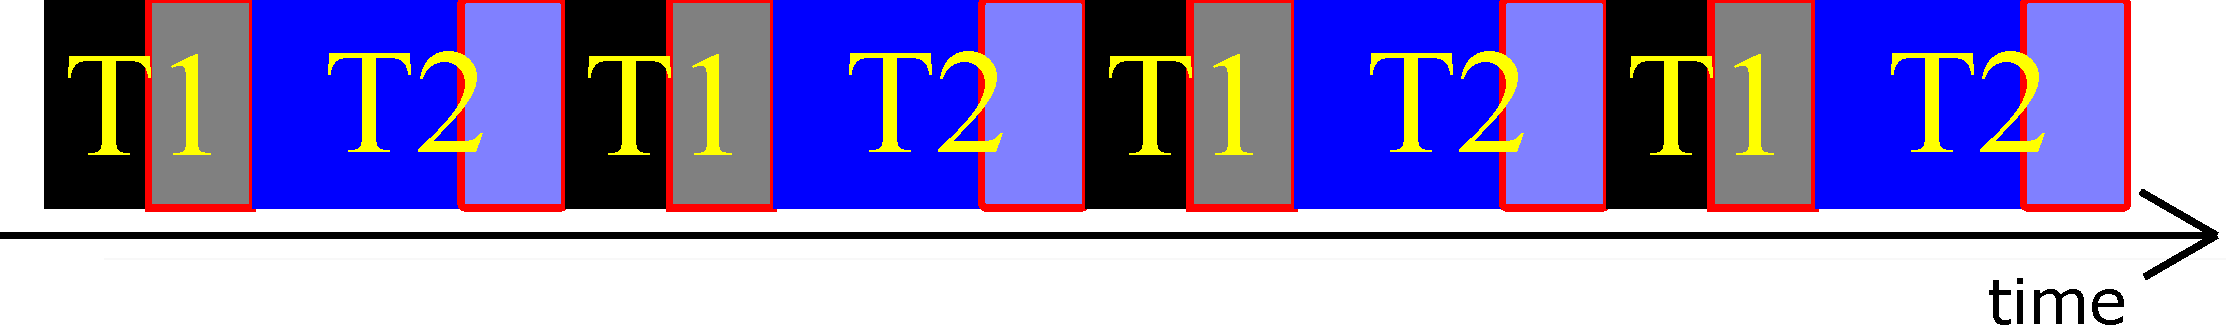
\includegraphics[width=\textwidth]{Figures/real-time-sched-2}

\onslide<4>{\centering \hilightA{Economic need for trading off guarantees for utilization}}

\end{frame}


%%%%%%%%%%%%%%%%%%%%%%%%%%%%%%%%%%%%%%%%%%%%%%%%%%%%%%%%%%%%%%%%%%%%%%%%%%%%%%
\subsection{Full-Scale Mode Switches}

\begin{frame}{Mixed Criticality Levels}

\begin{minipage}{\textwidth}
\begin{block}{Worst-Case Execution Time Estimates}<2->
\begin{itemize}
    \item<3-> Various components are validated against various assumptions
    \item<4-> The stricter assumptions, the longer estimated WCET
\end{itemize}
\end{block}

\vfill

\begin{block}{Criticality Levels of Tasks}<5->
\begin{itemize}
    \item<6-> Strictness of assumptions
    \item<7-> Ordered set of levels
\end{itemize}
\end{block}
\end{minipage}

\end{frame}

\begin{frame}{Mixed-Criticality Scheduling with Criticality Mode Switches}

\pause
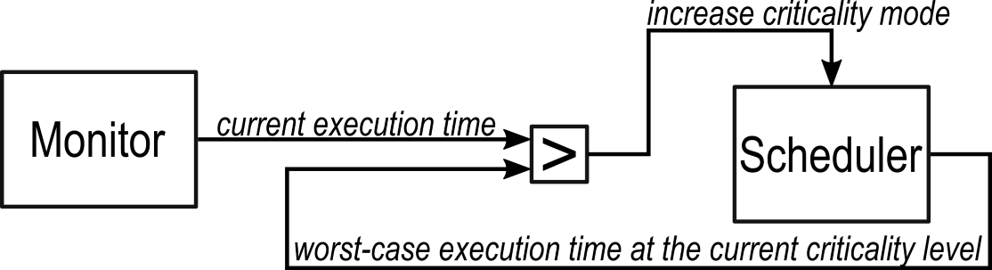
\includegraphics[width=\textwidth]{Figures/mixed-crit-sched-robin}
\pause
\begin{itemize}[<+->]
    \item Start system in the lowest criticality mode
    \item Schedule tasks with criticality not below the current criticality mode
    \item Monitor whether execution violates current assumptions
    \item Switch to higher criticality mode for stricter assumptions
\end{itemize}

\end{frame}


\begin{frame}{Mixed-Criticality Scheduling with Mode Switches}

\only<1-2>{%
\begin{minipage}{\textwidth}
\begin{block}{Task Set $HI$}
\begin{tabular}{cccc}
\textbf{Task}&\textbf{Period}&\textbf{Deadline}&\textbf{WCET}\\ \hline
$T1$&$10$&$5$&$4$\\
$T2$&$10$&$10$&$6$
\end{tabular}
\end{block}

\onslide<2>
\begin{block}{Task Set $LO$}
\begin{tabular}{cccc}
\textbf{Task}&\textbf{Period}&\textbf{Deadline}&\textbf{WCET}\\ \hline
$T1$&$10$&$5$&$2$\\
$T2$&$10$&$10$&$4$\\
$T3$&$10$&$9$&$3$
\end{tabular}
\end{block}
\end{minipage}
}

\only<3->{%
\begin{minipage}{\textwidth}
\begin{block}{Mixed-Criticality Task Set}
\begin{tabular}{ccccc}
\textbf{Task}&\textbf{CL}&\textbf{Period}&\textbf{Deadline}&\textbf{WCET}\\ \hline
$T1$&$HI$&$10$&$5$&$[2,4]$\\
$T2$&$HI$&$10$&$10$&$[4,6]$\\
$T3$&$LO$&$10$&$9$&$[3]$
\end{tabular}
\end{block}

\bigskip

\includegraphics<4>[width=\textwidth]{Figures/mixed-crit-sched-1}
\includegraphics<5>[width=\textwidth]{Figures/mixed-crit-sched-2}
\includegraphics<6>[width=\textwidth]{Figures/mixed-crit-sched-3}
\includegraphics<7>[width=\textwidth]{Figures/mixed-crit-sched-4}

\onslide<6->{\centering \hilightA{Ignoring $LO$ criticality tasks in $HI$ mode}}

\end{minipage}
}

\end{frame}

\begin{frame}{Limitations of Mode Switching Scheduling}

\pause
\begin{block}{Static Verification}\onslide<2->
\begin{itemize}
    \item<3-> Timing guarantees for each mode
    \item<4-> \hilightA{No link to requirements of safety standards}
\end{itemize}
\end{block}

\begin{block}{Runtime Robustness}\onslide<2->
\begin{itemize}
    \item<5-> Switching mode to restrict assumptions as necessary
    \item<6-> \hilightA{Ignoring low-criticality tasks}
    \item<7-> \hilightA{Returning to low-criticality mode}
\end{itemize}
\end{block}

\end{frame}


%%%%%%%%%%%%%%%%%%%%%%%%%%%%%%%%%%%%%%%%%%%%%%%%%%%%%%%%%%%%%%%%%%%%%%%%%%%%%%
\subsection{Memory Access Budgeting}

\begin{frame}{Memory Accesses and Execution Time}

\begin{block}{Cache Misses}<2->
\begin{itemize}
    \item<3-> Memory needs to be accessed
    \item<4-> Critical tasks may be penalized by interference
\end{itemize}
\end{block}

\begin{block}{Limited Interference for Critical Tasks}<5->
\begin{itemize}
    \item<6-> Reduce WCET of critical tasks by limiting interference
    \item<7-> Budget of cache misses for non-critical tasks (cores)
    \item<8-> Suspend execution of tasks with depleted budget
\end{itemize}
\end{block}

\vfill

\onslide<9->{\centering \hilightB{Can be generalized to any shared resource}}

\end{frame}

\begin{frame}{Memory Access Budgeting}

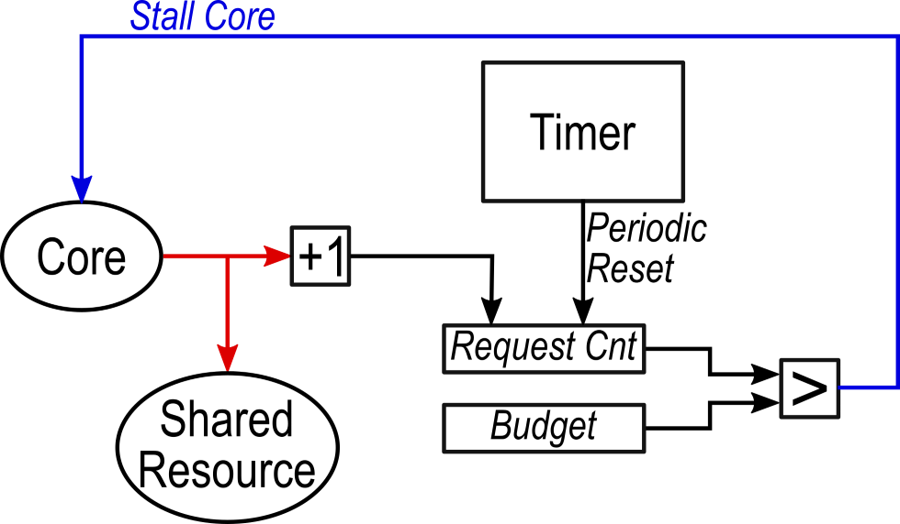
\includegraphics[width=\textwidth]{Figures/budgeting-robin}

\end{frame}


\begin{frame}{Memory Access Budgeting -- Pros and Cons}


\begin{block}{Pros}
\begin{itemize}
    \item<2-> Low overhead on COTS
    \begin{itemize}
        \item<3-> Performance counters
        \item<3-> Interprocessor interrupts
    \end{itemize}
\end{itemize}
\end{block}

\vfill

\begin{block}{Cons}
\begin{itemize}
    \item<4-> Limited to $2$ levels, critical and non-critical
    \item<5-> No general algorithm for deriving budgets
    \item<6-> Not scaling with the number of non-critical cores
\end{itemize}
\end{block}

\end{frame}

%%%%%%%%%%%%%%%%%%%%%%%%%%%%%%%%%%%%%%%%%%%%%%%%%%%%%%%%%%%%%%%%%%%%%%%%%%%%%%
\subsection{Execution Time Monitoring}

\begin{frame}{Monitoring Execution Time and Remaining WCET}

\begin{block}{WCET and Observation Points for Critical Tasks}<2->
\begin{itemize}
    \item<3-> Remaining WCET for each observation point
    \item<4-> Worst-case interference between observation points
\end{itemize}
\end{block}

\vfill

\begin{block}{Safety Condition at each Observation Point}<5->
The critical task will not miss its deadline even if worst-case happens until the next observation point
\end{block}

\end{frame}

\begin{frame}{Execution Time Monitoring}

Evaluate safety condition at each observation point:

\vfill

\begin{tabular}{lp{2pt}cl}
\onslide<2->{\color{olive}code segment $k-$}&&&\onslide<4->{\color{olive}execution time}\\
\onslide<3->{observation point $k$}&&&\\
\onslide<2->{\color{orange}code segment $k$}&&\onslide<4->{$+$}&\onslide<4->{\color{orange}$WCET_{interference}(k, k+1)$}\\
\onslide<3->{observation point $k+1$}&&&\\
\onslide<2->{\color{red}code segment $k+$}&&\onslide<4->{$+$}&\onslide<4->{\color{red}$WCET_{isolation}(k+1, end)$}\\
&&&\\
&&\onslide<4->{$+$}&\onslide<4->{\color{purple}observation overhead}\\
&&&\\
&&\onslide<4->{$<$}&\onslide<4->{deadline}
\end{tabular}

\vfill

\onslide<5->{%
Suspend non-critical tasks if safety condition does not hold.
}

\end{frame}


\begin{frame}{Execution Time Monitoring -- Pros and Cons}

\begin{block}{Pros}
\begin{itemize}
    \item<2-> Code instrumentation is easy to implement on COTS
    \item<3-> Monitoring execution time limits pessimism
    \item<4-> Evaluating condition at observation points limits pessimism
\end{itemize}
\end{block}

\vfill

\begin{block}{Cons}
\begin{itemize}
    \item<5-> Limited to $2$ levels, critical and non-critical
    \item<6-> Large execution time overhead of monitoring
\end{itemize}
\end{block}

\end{frame}


%%%%%%%%%%%%%%%%%%%%%%%%%%%%%%%%%%%%%%%%%%%%%%%%%%%%%%%%%%%%%%%%%%%%%%%%%%%%%%
\subsection{Workload Arrival Monitoring}

\begin{frame}{Workload Arrival Functions}

\end{frame}

\begin{frame}{Workload Arrival Monitoring}

\end{frame}


\begin{frame}{Workload Arrival Monitoring -- Pros and Cons}

\end{frame}

%%% Local Variables:
%%% mode: latex
%%% TeX-master: "slides"
%%% End:

\section{Mixed Criticality Bus Arbiters}

%%%%%%%%%%%%%%%%%%%%%%%%%%%%%%%%%%%%%%%%%
\begin{frame}{Goals of Mixed-Criticality Communication Protocols}

\vspace{-0.3cm}

\visible<1->{
\begin{block}{Resource Utilization}
\begin{itemize}
\item Enable the derivation of tight latency bounds for guaranteed latency traffic
\item Analyzable in terms of schedulability
\end{itemize}
\end{block}
}

\visible<2->{
\begin{block}{Quality of Service}
\begin{itemize}
\item Reduce the average latency of best-effort traffic
\item Not applicable to guaranteed latency traffic
\end{itemize}
\end{block}
}

\visible<3->{
\begin{block}{Scalability}
\begin{itemize}
\item Scale well with the number of bus masters or NoC nodes
\end{itemize}
\end{block}
}

\end{frame}
%%%%%%%%%%%%%%%%%%%%%%%%%%%%%%%%%%%%%%%%%%%%%%%%%%%%%%%
\begin{frame}{TDMA-RR Dual Layer Arbiter}

\vspace{-0.3cm}

\begin{itemize}
\item First layer : TDMA for critical bus masters
\item Second layer : RR for non-critical bus masters
\end{itemize}

\vspace{0.3cm}

\includegraphics<1>[width=\textwidth]{TDMA-RR_Arbiter_Grey.png}
\includegraphics<2>[width=\textwidth]{TDMA-RR_Arbiter.png}

\end{frame}
%%%%%%%%%%%%%%%%%%%%%%%%%%%%%%%%%%%%%%%%%%%%%%%%%%%%%%%
\begin{frame}{Criticality- and Requirement-Aware Bus Arbiter}

\vspace{-0.3cm}

\begin{itemize}
\item \visible<1-> First layer : arbitration between criticality classes
\item \visible<1-> Second layer : arbitration between tasks of the elected criticality class
\item \visible<2-> {Both layers are Weighted Harmonic RR}
\end{itemize}

\visible<2->{
\begin{block}{Weighted Harmonic Round Robin}
\begin{itemize}
\item Bus control granted for 1 request only
\item Each master can get several slots per period
\item Slots are evenly distributed
\end{itemize}
\end{block}
}

\end{frame}

\begin{frame}{CArb - Example}

\vspace{-0.3cm}
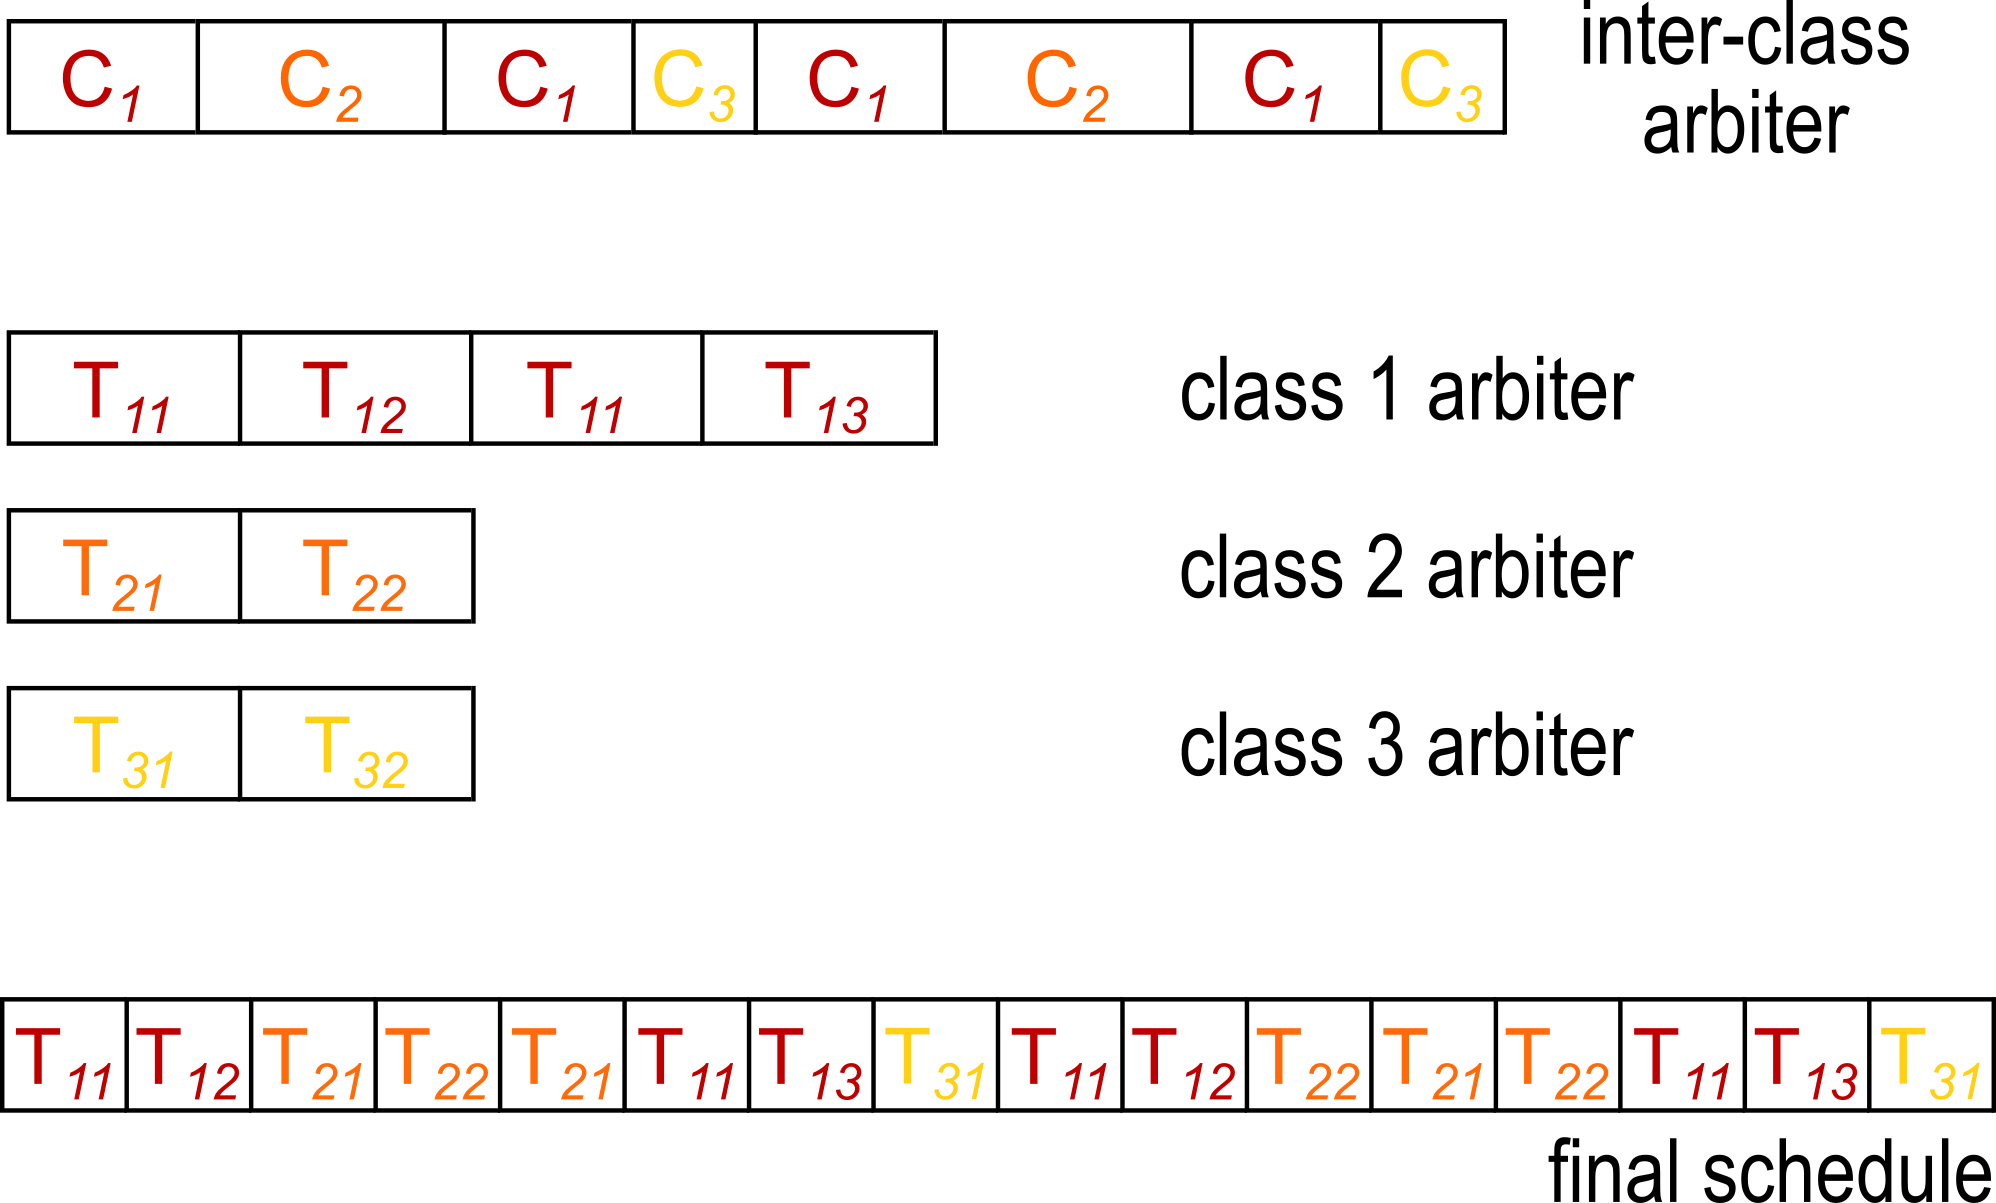
\includegraphics[width=\textwidth]{CArb1.png}

\end{frame}

\begin{frame}{CArb - Arbiter-level Mode Switch}

\visible<1->{
\(\text{WCET}_{total}(\text{T}_{\textit{13}}) < exec\_time(\text{T}_{\textit{13}})\)\\
\(\to\) Drop low-critical tasks, system-wide mode switch
\vspace{0.5 cm}
}

\visible<2->{
\(\text{WCET}_{iso}(\text{T}_{\textit{13}}) < exec\_time(\text{T}_{\textit{13}}) < \text{WCET}_{total}(\text{T}_{\textit{13}})\)\\
\(\to\) Cut interference, arbiter-level mode switch

\begin{center}

\includegraphics[width=0.25\textwidth]{CArb2.png}
\end{center}
}

\visible<3->{
If \(exec\_time(\text{T}_{\textit{13}}) - \text{WCET}_{iso}(\text{T}_{\textit{13}}) < \textit{threshold}\)\\
\(\to\) Cut only part of the interference

\begin{center}

\includegraphics[width=0.90\textwidth]{CArb3.png}
\end{center}
}

\end{frame}


%%% Local Variables:
%%% mode: latex
%%% TeX-master: "slides"
%%% End:

\section{Mixed Criticality NoCs}

%%%%%%%%%%%%%%%%%%%%%%%%%%%%%%%%%%%%%%%%%%%%%%%%%%%%%%%
\begin{frame}{Wormhole Protocol for Mixed-Criticality}

\begin{center}
\includegraphics<1>[width=0.8\textwidth]{WPMCRouterGrey.png}
\includegraphics<2>[width=0.8\textwidth]{WPMCRouter.png}
\end{center}

\end{frame}

\begin{frame}{WPMC-Flood}
\begin{center}
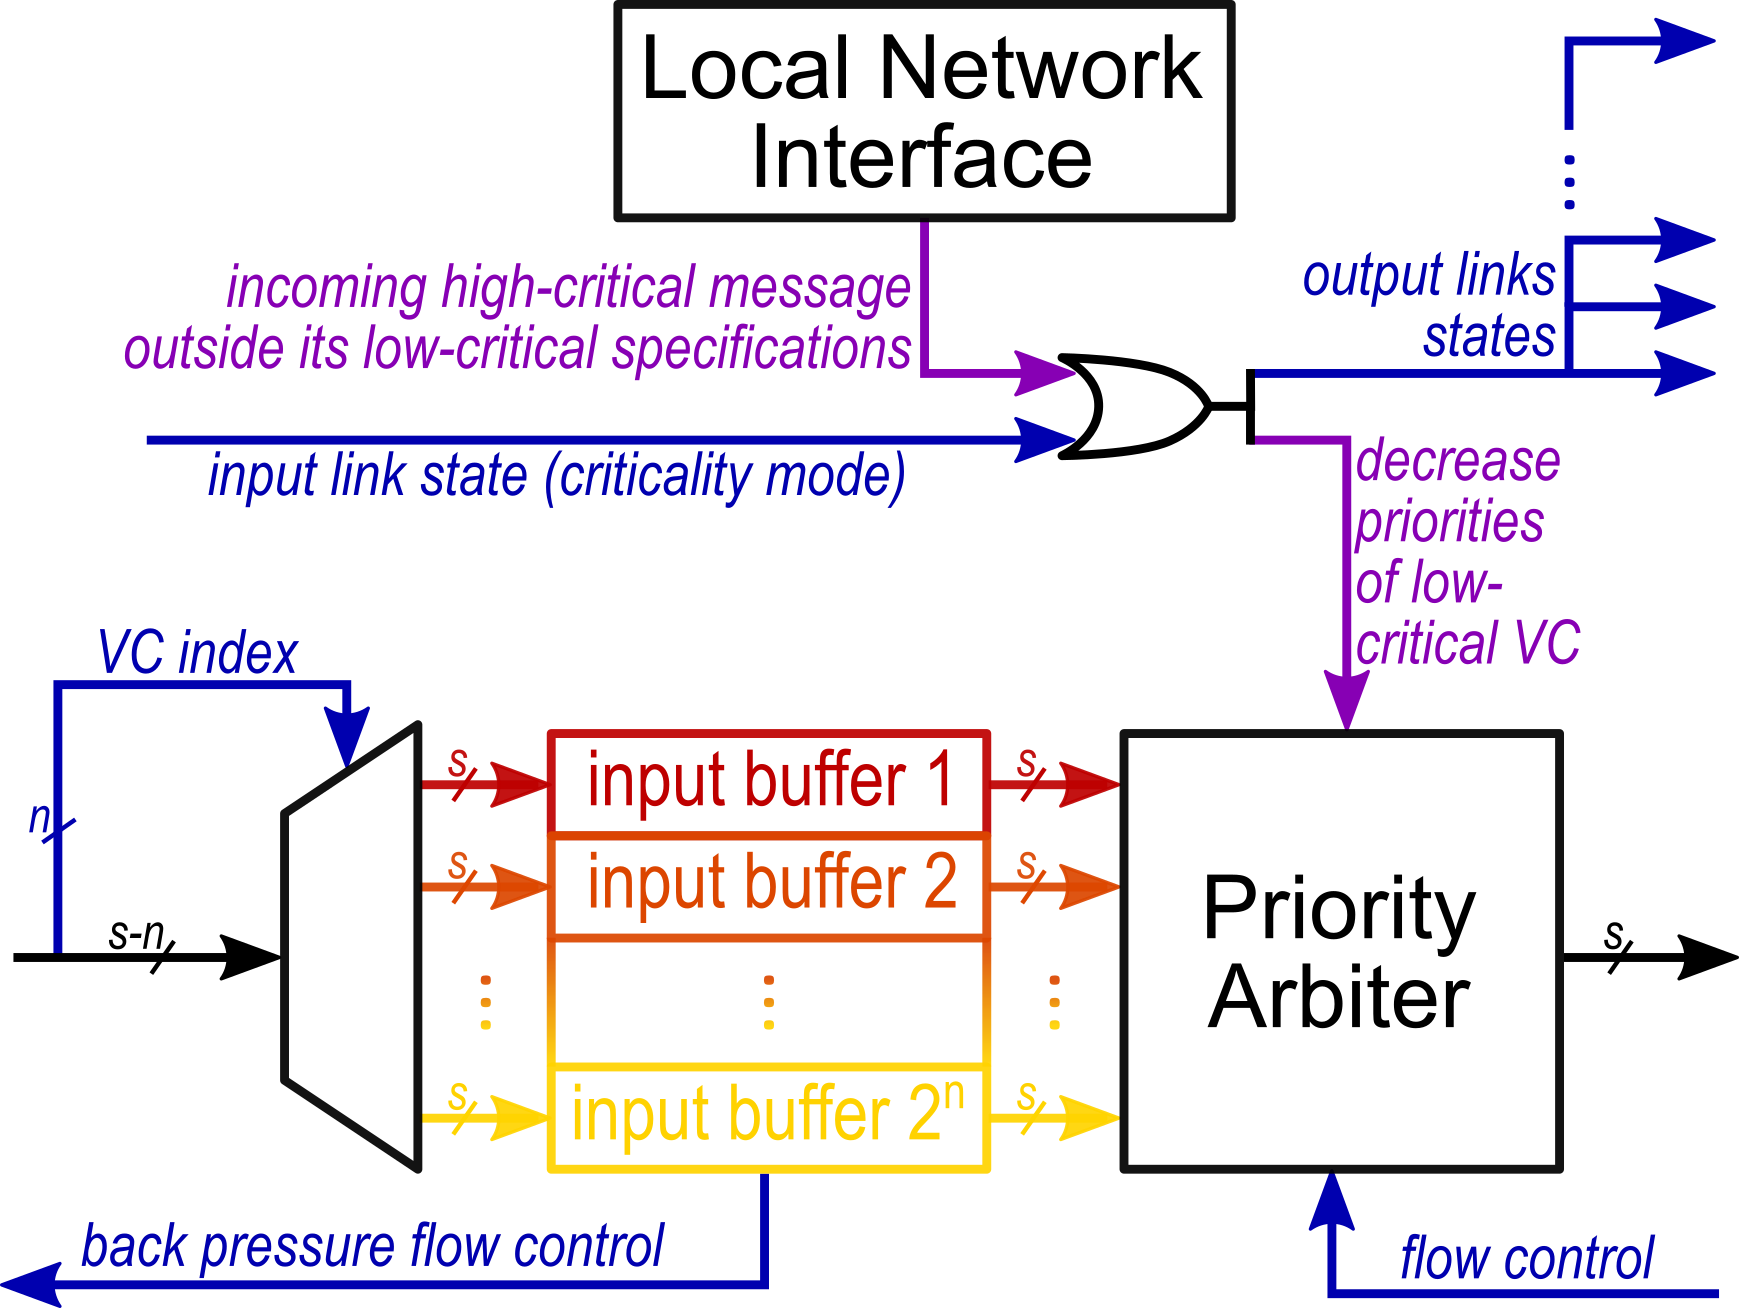
\includegraphics[width=0.8\textwidth]{WPMCFloodRouter.png}
\end{center}
\end{frame}
%%%%%%%%%%%%%%%%%%%%%%%%%%%%%%%%%%%%%%%%%%%%%%%%%%%%%%%
\begin{frame}{Wormhole with Blocking Counter}
\vspace{-0.3cm}
The header flit of critical messages contains a \textit{Blocking Counter} field.
\vspace{1cm}

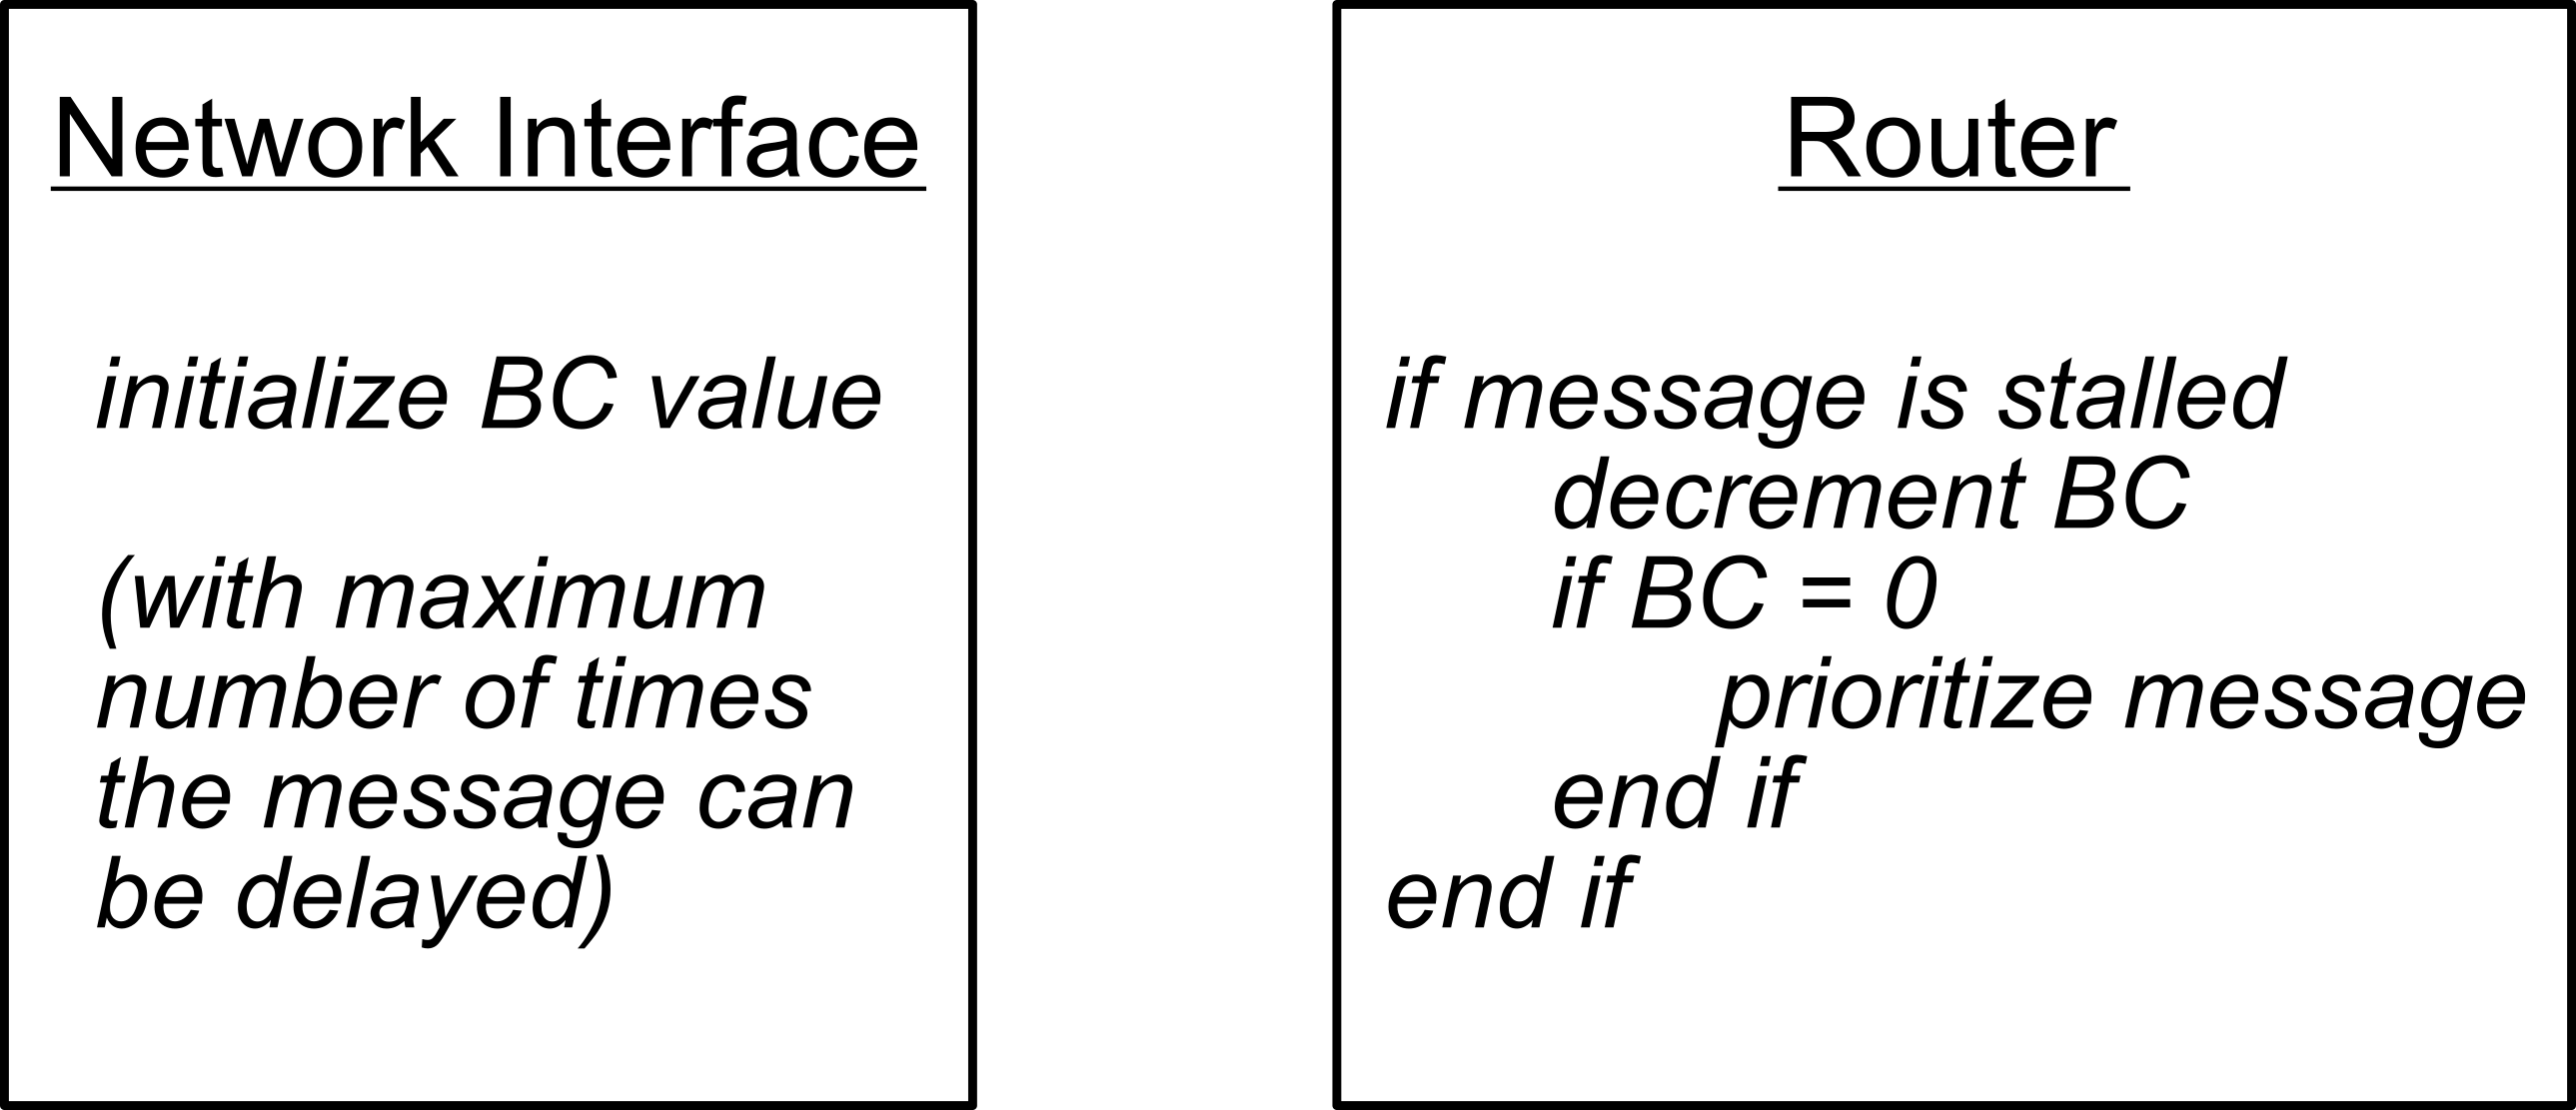
\includegraphics[width=0.85\textwidth, center]{BC.png}
\end{frame}
%%%%%%%%%%%%%%%%%%%%%%%%%%%%%%%%%%%%%%%%%%%%%%%%%%%%%%%
\begin{frame}{Adaptive Routing}
\begin{columns}

\begin{column}{0.4\textwidth}
\includegraphics<1>[width=0.85\textwidth, right]{AR1.png}
\includegraphics<2>[width=0.85\textwidth, right]{AR2.png}
\end{column}

\begin{column}{0.6\textwidth}
\begin{itemize}
\item <1-> Message BE1\\
Path list : \{(1,2), (2,2)\}, \{(1,2), (1,1), (2,1), (2,2)\}
\vspace{0.5cm}
\item <2-> Message C1\\
Path list: \{(1,2), (2,2)\}
\end{itemize}
\end{column}

\end{columns}
\end{frame}

\begin{frame}{Adaptive Routing - Control Scheme}
\begin{center}
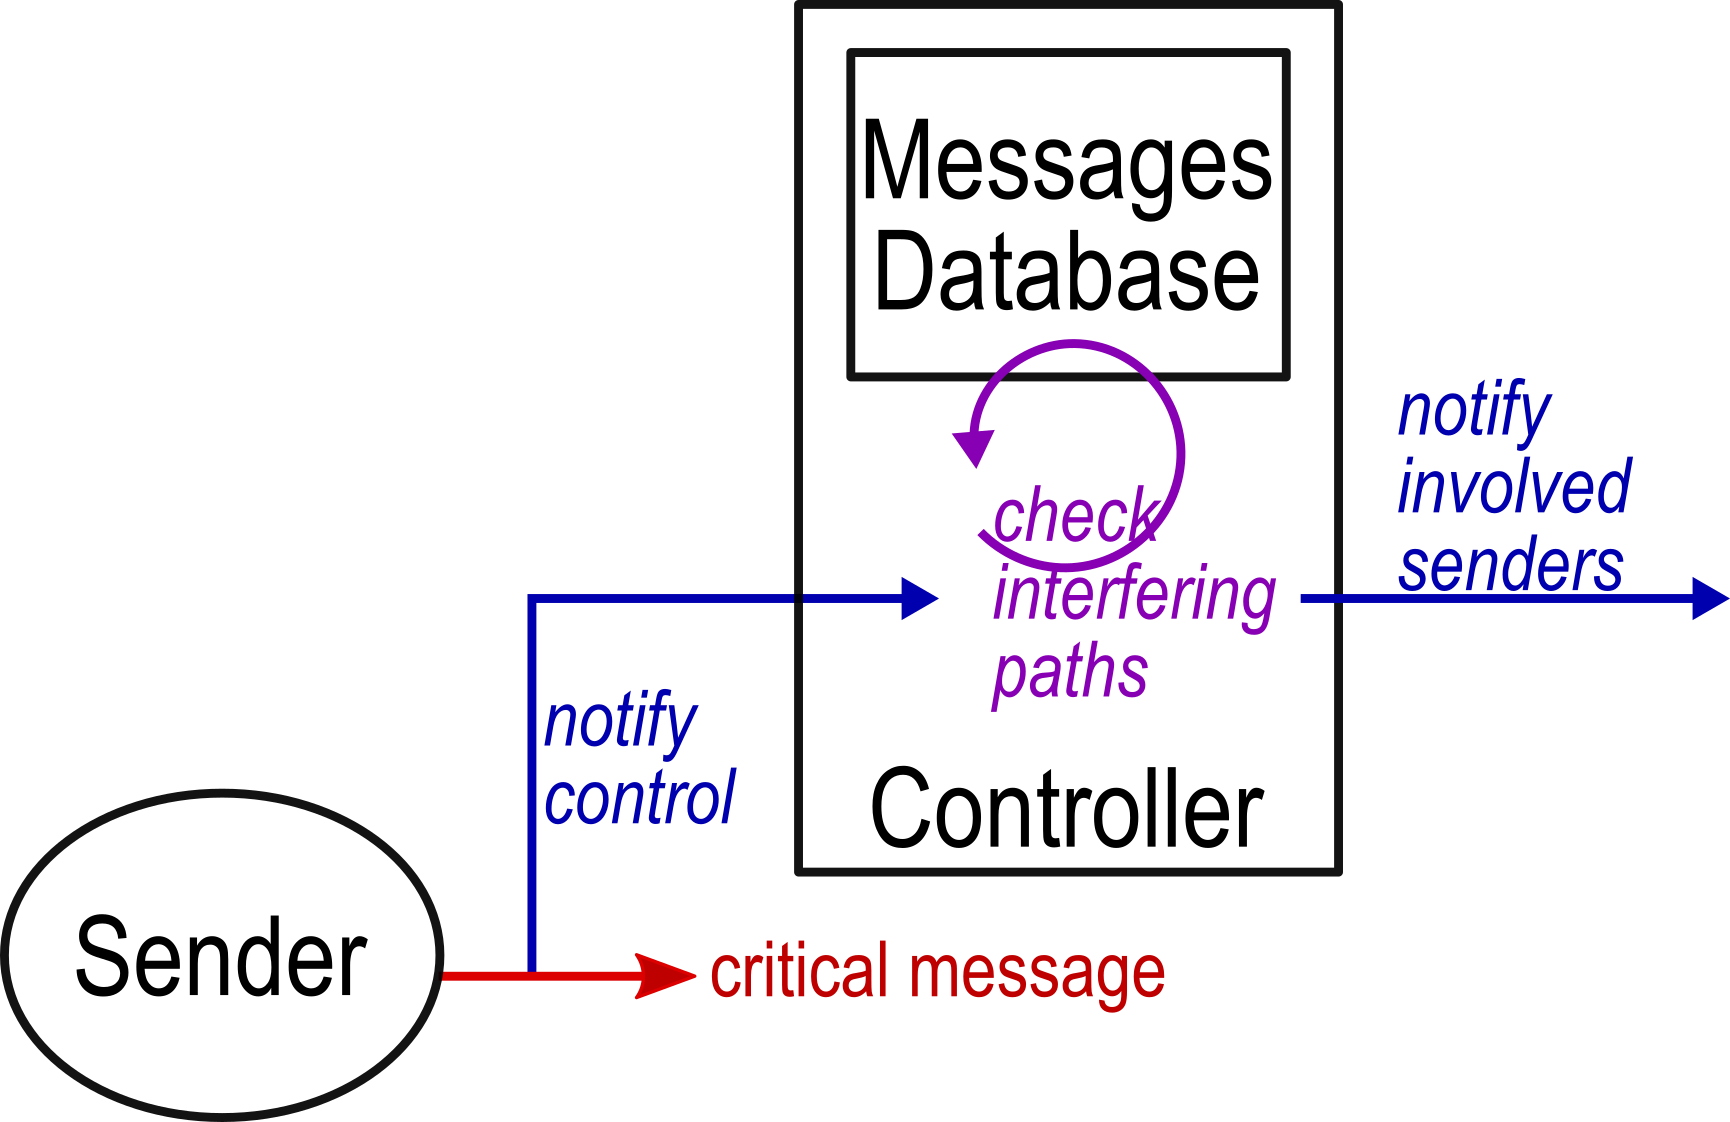
\includegraphics[width=0.75\textwidth]{ARCL.png}
\end{center}

\end{frame}

%%% Local Variables:
%%% mode: latex
%%% TeX-master: "slides"
%%% End:

\section{Mixed Criticality Architectures}

%%%%%%%%%%%%%%%%%%%%%%%%%%%%%%%%%%%%%%%%%
% \begin{frame}{Integrated Dependable Architecture for Many-Cores}

% \begin{itemize}
% \item Resources are distributed over Tiles, which are groups of resources sharing one NoC access point
% \item Tiles communicate with each other through an Address Translation Table
% \item A budgeting mechanism limits the number of messages sent to each local address
% \item One special tile serves as System Controller
% \begin{itemize}
% \item The SC is responsible for ATT configuration
% \item The SC can stall, reset, or disable any tile
% \end{itemize}
% \end{itemize}

%\end{frame}

\begin{frame}{Integrated Dependable Architecture for Many-Cores}

\begin{center}
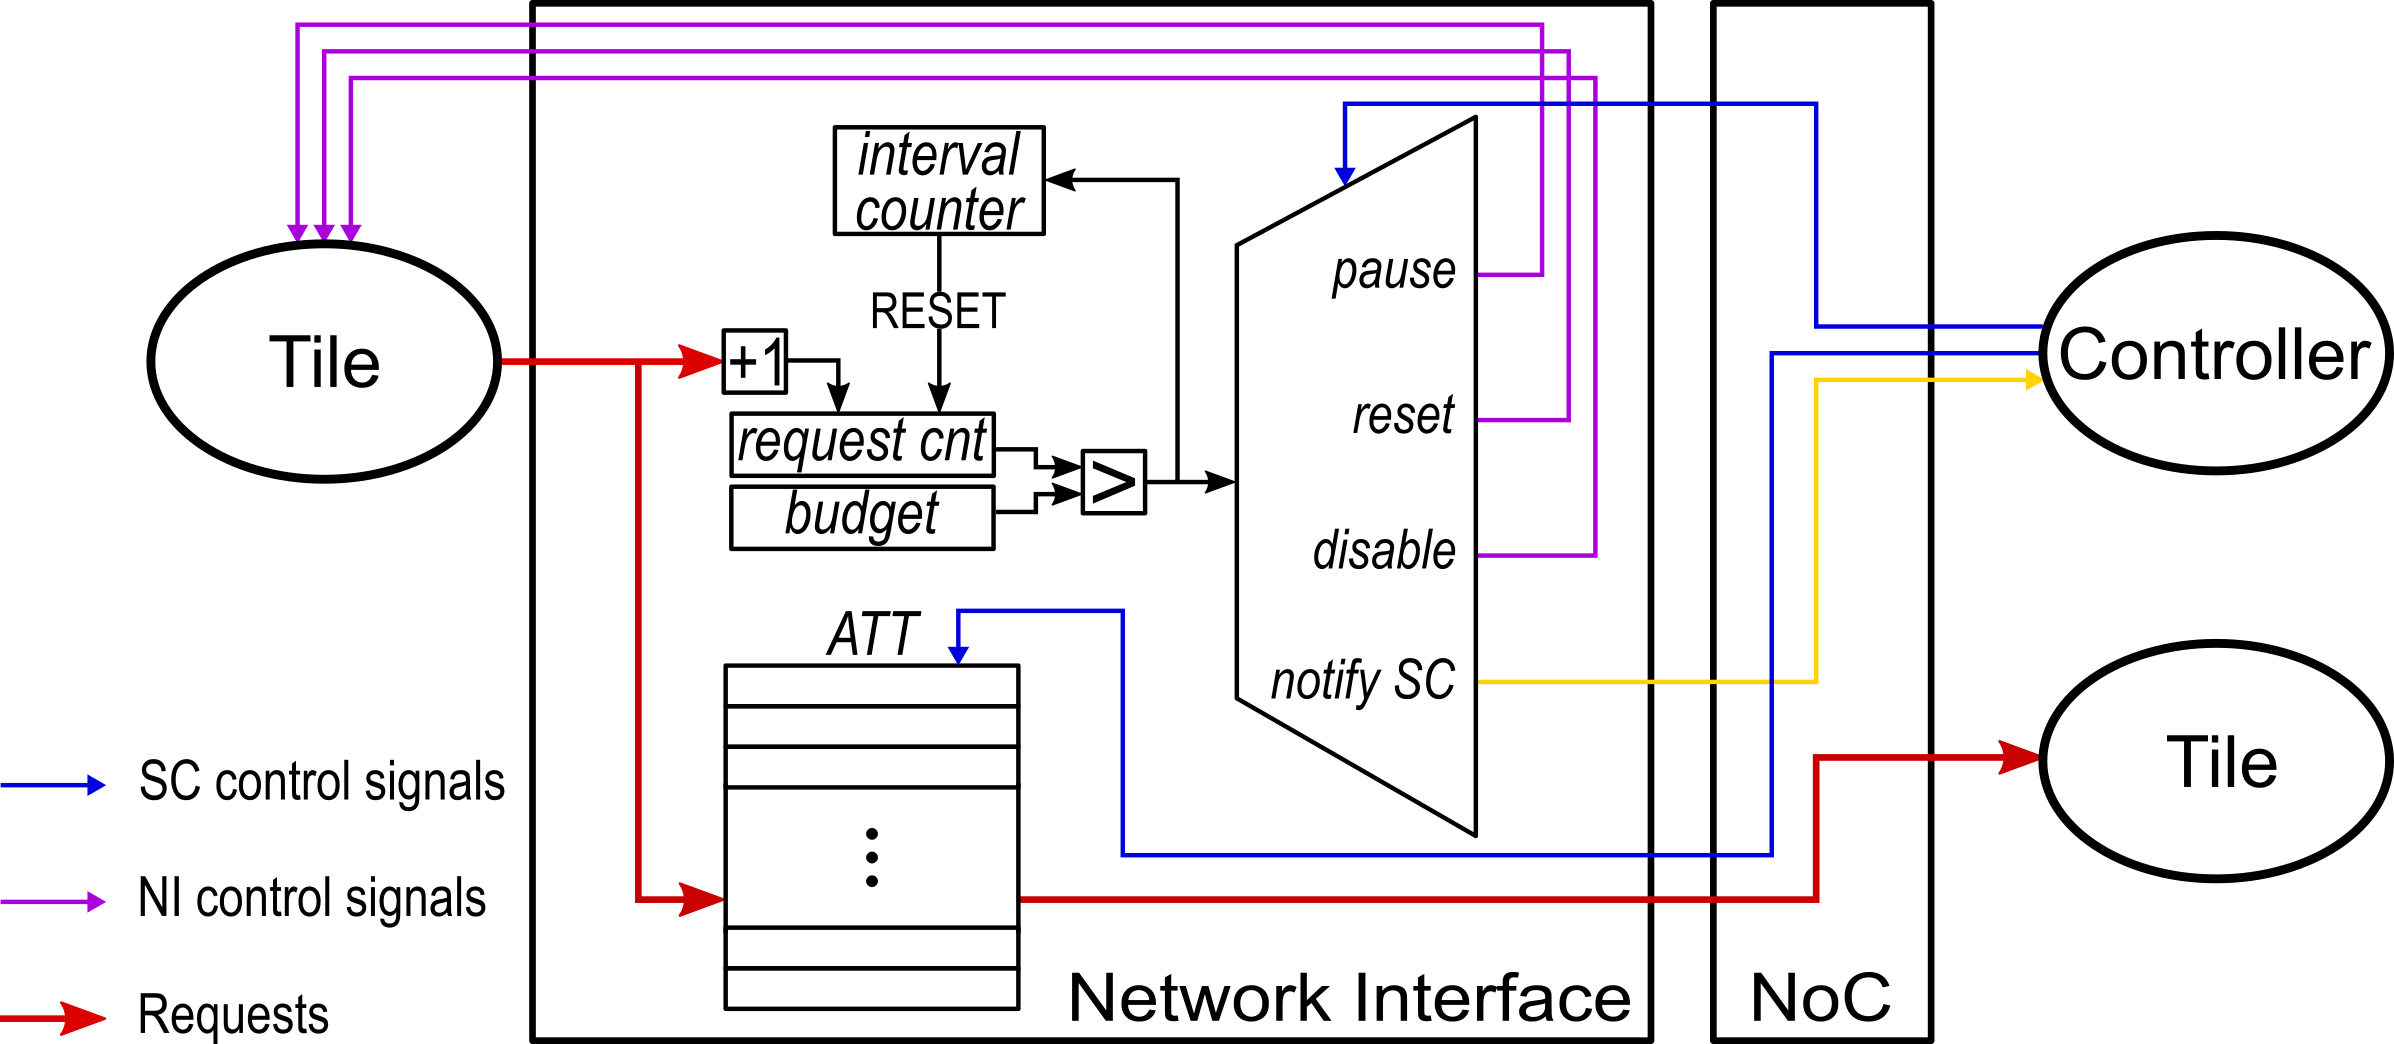
\includegraphics[width=\textwidth]{IDAMC.png}
\end{center}

\end{frame}
%%%%%%%%%%%%%%%%%%%%%%%%%%%%%%%%%%%%%%%%%
\begin{frame}{Integrating Scheduling and Data mapping}

Hardware model:

\begin{itemize}
\item \visible <1-> {16 Clusters}
\item \visible <2-> {Each containing 16 cores, 3 NoC interfaces, and 16 SRAM banks}
\item \visible <3-> {Each SRAM bank has its own dedicated controller, which arbitrates between all cores and interfaces}
\visible <4-> {
\begin{itemize}
\item NoC receiver interface always has priority
\item RR arbitration is performed between other components
\end{itemize}}
\end{itemize}

\end{frame}

\begin{frame}{Integrate Scheduling and Data mapping}

Software model:

\begin{itemize}
\item \visible<1-> {Independent task set and scheduler for each cluster}
\item \visible<2-> {Criticality mode switch}
\item \visible<3-> {Scheduling data:
\begin{itemize}
\item Execution times \textbf{without memory accesses}
\item Number of memory accesses
\item Dependency graph
\end{itemize}}
\item \visible<4-> {Tasks of different criticality cannot be scheduled on the same time frame}
\item \visible<5-> {Joint computation of task schedule and data mapping to SRAM banks}

\end{itemize}
\end{frame}

\begin{frame}{Controlling interference from other tiles}

When a task requires data to be fetched through the NoC

\vspace{1cm}

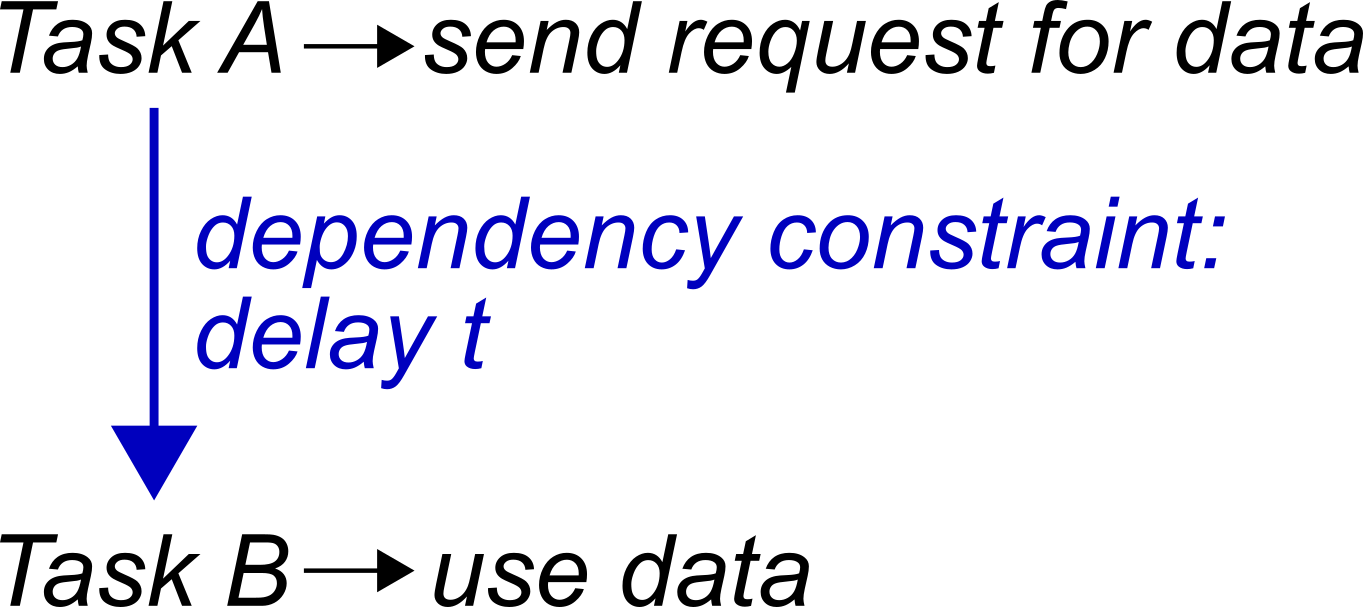
\includegraphics[width=0.5\textwidth]{initDataFetch.png}

\vspace{0.5cm}

\(t = 2* \text{NoC worst-case latency} + \text{resource worst-case response time}\)

\end{frame}

\begin{frame}{Higher level modeling - Resource Servers}
\begin{itemize}
\item \visible <1-> {A resource server "encapsulates" the access to a resource}
\item \visible <2-> {This can allow to consider only the server and the requesting component in modeling}
\item \visible <3-> {The resource itself and the interfering components can be laid aside \textbf{provided the inter-process communication protocol is adequate}}
\item \visible <4-> {For MCS, the IPC protocol should also take criticality into account}
\end{itemize}
\end{frame}

\begin{frame}{Resource Server for MCS}

\includegraphics<1>[width=\textwidth]{ResourceServerGrey.png}
\includegraphics<2>[width=\textwidth]{ResourceServerGrey2.png}
\includegraphics<3>[width=\textwidth]{ResourceServer.png}

\end{frame}
%%% Local Variables:
%%% mode: latex
%%% TeX-master: "slides"
%%% End:

\section{Conclusions}

%%%%%%%%%%%%%%%%%%%%%%%%%%%%%%%%%%%%%%%%%
\begin{frame}{Mixed Criticality Systems}
  
  \begin{itemize}[<+->]
  \item Response to a pressing industrial need:
  
    \begin{itemize}
    \item How to provide safety and real-time guarantees in efficient
      implementations?
    \end{itemize}
  \item Mixed Criticality scheduling Theory;
    
    \begin{itemize}
    \item Design time verification;
    \item Run-time robustness, when the system violates assumptions;
    \end{itemize}
  \item Providing sound mechanisms for sharing:
    
    \begin{itemize}
    \item Processing elements;
    \item Buffers, caches, memory;
    \item I/O: Pins, drivers;
    \item \hilightB{Communication.}
    \end{itemize}
  \end{itemize}
\end{frame}


%%% Local Variables:
%%% mode: latex
%%% TeX-master: "slides"
%%% End:




%%%%%%%%%%%%%%%%%%%%%%%%%%%%%%%%%%%%%%%%%%%%%%%%%%%%%%%%%%%%%%%%%%%%%%%%%%%%%



%%%%%%%%%%%%%%%%%%%%%%%%%%%%%%%%%%%%%%%%%%%%%%%%%%%%%%%
\begin{frame}{}

  \centering\Huge
  ?` Questions ?
\end{frame}

%%%%%%%%%%%%%%%%%%%%%%%%%%%%%%%%%%%%%%%%%%%%%%%%%%%%%%%%%%%%%%%%%%%%%%%%%%%%% 
%%%%%%%%%%%%%%%%%%%%%%%%%%%%%%%%%%%%%%%%%%%%%%%%%%%%%%%%%%%%%%%%%%%%%%%%%%%%%

\end{document}


%%% Local Variables:
%%% mode: latex
%%% TeX-master: t
%%% End:
